\section{Results}
We organize the evaluation around four questions: whether BPGS is robust to explicit scale perturbations, whether that robustness transfers to a standard dense-prediction benchmark, which parts of the method matter in ablation, and whether the method remains competitive outside the synthetic stress setting.

\subsection{Robustness to loss-scale mismatch}
Figure~\ref{fig:stress_summary} separates two perturbation types. The right column isolates pure post-hoc loss rescaling, where only the numerical scale changes. In that setting, BPGS is effectively invariant: its macro score stays at 0.777, 0.784, 0.781, and 0.778 from $\times 1$ through $\times 1000$ (Table~\ref{tab:stress_rescaling} and Appendix Figure~\ref{fig:appendix_rescaling}). Proposition~\ref{prop:invariance} shows that the normalized weights themselves are invariant under this rescaling when the safeguards are inactive; the table is an empirical diagnostic of the resulting training behavior. Kendall-style uncertainty weighting starts slightly higher at $\times 1$ but drops monotonically to 0.637 at $\times 1000$, while UWSO improves modestly from a much weaker starting point.

\begin{table}[t]
\centering
\caption{Pure loss rescaling (06): Macro Score across scale factors. Mean $\pm$ std over 3 seeds.}
\label{tab:stress_rescaling}
\resizebox{\columnwidth}{!}{%
\begin{tabular}{l c c c c}
\toprule
Method & $\times{1}$ & $\times{10}$ & $\times{100}$ & $\times{1000}$ \\
\midrule
Kendall & $\mathbf{0.780 \pm 0.007}$ & $0.769 \pm 0.013$ & $0.714 \pm 0.017$ & $0.637 \pm 0.015$ \\
UWSO & $0.622 \pm 0.073$ & $0.674 \pm 0.036$ & $0.688 \pm 0.035$ & $0.681 \pm 0.014$ \\
BPGS & $0.777 \pm 0.012$ & $\mathbf{0.784 \pm 0.008}$ & $\mathbf{0.781 \pm 0.001}$ & $\mathbf{0.778 \pm 0.006}$ \\
\bottomrule
\end{tabular}
}
\end{table}

\paragraph{Normalization is not sufficient.}\label{sec:norm_ablation}
On a separate three-seed diagnostic, L1-normalized Kendall improves over unnormalized Kendall at
$\times1000$ (0.689 versus 0.658) but still falls by 0.105 from $\times1$ to $\times1000$;
BPGS falls by 0.004 (Appendix~\ref{app:norm_ablation}). The completed diagnostic uses a different
seed set from the main rescaling table, so this comparison is interpreted as evidence that
normalization alone is insufficient, not as a seed-matched estimate of the main-table gap.

\begin{figure*}[t]
\centering
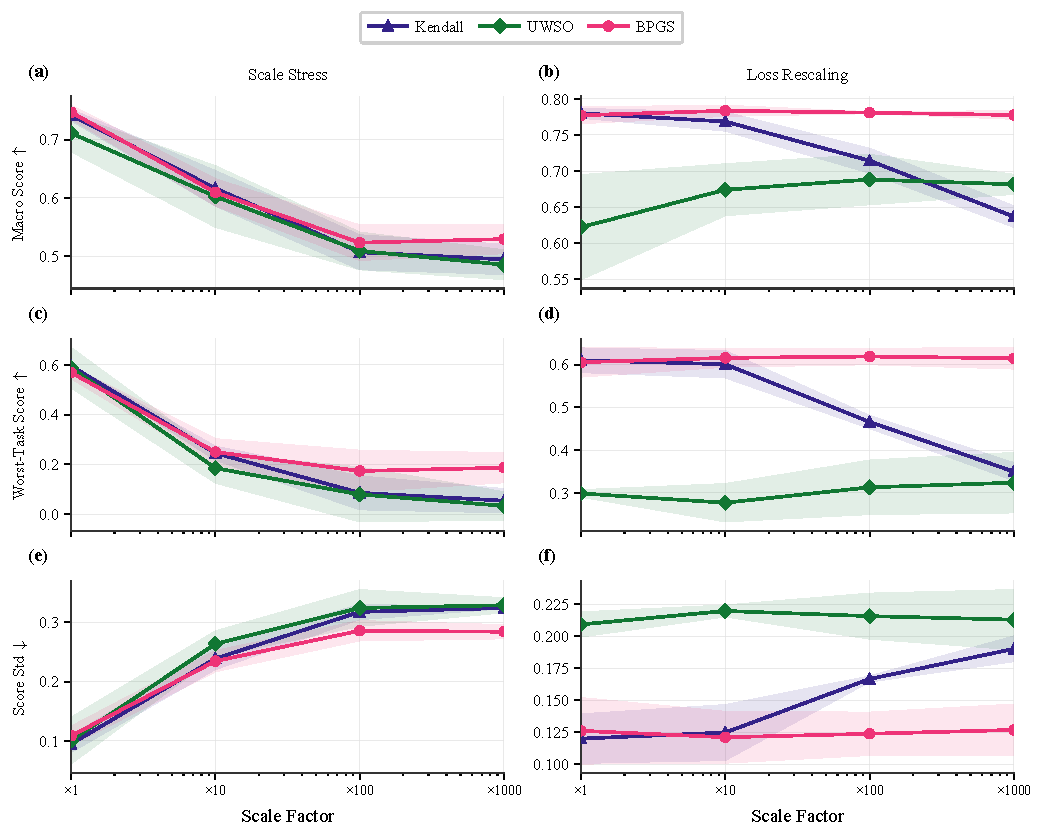
\includegraphics[width=\textwidth]{data/stress/combined/figures/pdf/stress_robustness_summary.pdf}
\caption{Synthetic robustness diagnostics under scale mismatch. Left column: scale stress, where performance is evaluated as task scales become increasingly imbalanced. Right column: pure loss rescaling, where only the reported magnitude changes. BPGS remains nearly invariant under pure rescaling and retains the strongest macro score at the largest scale-stress factors.}
\label{fig:stress_summary}
\end{figure*}

The left column of Figure~\ref{fig:stress_summary} is the harder test because the perturbation changes the optimization problem rather than only its units. All three methods degrade as the factor increases, but BPGS is best at $\times 1$, $\times 10$, $\times 100$, and $\times 1000$, reaching 0.543 at $\times 1000$ versus 0.499 for Kendall and 0.494 for UWSO. The relative drop from $\times 1$ to $\times 1000$ is 27.0\% for BPGS, compared with 32.3\% for Kendall and 28.5\% for UWSO (Appendix Table~\ref{tab:degradation}; see also Appendix Figure~\ref{fig:appendix_scale_stress}). The BPGS--Kendall gap at $\times 1000$ is 0.043, or 1.07 combined standard deviations, so the updated 10-seed estimate is directionally stronger than the original 3-seed result but still should be read as a comparison of means rather than a formal significance test. In our experiments, this provides the strongest support for the bounded, batch-aware construction.

The heterogeneous mixed-stress study is less favorable to BPGS than the explicit scale-mismatch studies (Appendix Table~\ref{tab:stress_heterogeneous} and Appendix Figure~\ref{fig:appendix_heterogeneous}). Kendall and PCGrad attain higher macro scores in the noisy and conflict regimes, whereas BPGS gives the strongest worst-task score in the clean regime at 0.301 and remains far above the UWSO worst-task score of 0 throughout. We therefore interpret BPGS as a method targeted at loss-scale robustness rather than as a general solution to heterogeneous task interaction.

\subsection{Main NYUv2 benchmark}
Table~\ref{tab:nyuv2_main} shows that no method dominates every metric. Static achieves the best segmentation mIoU, and UWSO is strongest on the two surface-normal metrics. BPGS, however, gives the strongest depth results and a strong aggregate trade-off by the reported summary metrics: it attains the best absolute relative depth error (0.223), the best depth RMSE (0.790), the lowest total loss (1.891), and the highest $\Delta_M$ (0.078). The same trade-off pattern is visible in Appendix Figures~\ref{fig:appendix_nyuv2_bars}--\ref{fig:appendix_nyuv2_delta}.

\begin{table}[t]
\centering
\caption{NYUv2 dense prediction benchmark. All methods trained for 120 epochs. Final-epoch metrics reported as mean $\pm$ std over 3 seeds. $\Delta_M$ is computed against the Static baseline; the Nash-MTL value is derived from the reported mean metrics and is shown approximately.}
\label{tab:nyuv2_main}
\resizebox{\columnwidth}{!}{%
\begin{tabular}{l c c c c c c c}
\toprule
Method & mIoU $\uparrow$ & Abs Rel $\downarrow$ & RMSE $\downarrow$ & Angle $\downarrow$ & Within 11.25$^\circ$ $\uparrow$ & Total Loss $\downarrow$ & $\Delta_M$ $\uparrow$ \\
\midrule
Static & $\mathbf{0.341 \pm 0.006}$ & $0.239 \pm 0.000$ & $0.829 \pm 0.011$ & $35.934 \pm 2.055$ & $0.169 \pm 0.009$ & $1.992 \pm 0.033$ & $0.000 \pm 0.000$ \\
Kendall & $0.281 \pm 0.013$ & $0.229 \pm 0.001$ & $\underline{0.808 \pm 0.003}$ & $28.629 \pm 0.431$ & $0.231 \pm 0.007$ & $1.977 \pm 0.029$ & $0.022 \pm 0.000$ \\
UWSO & $0.294 \pm 0.007$ & $\underline{0.228 \pm 0.003}$ & $0.815 \pm 0.012$ & $\mathbf{26.110 \pm 0.383}$ & $\mathbf{0.271 \pm 0.007}$ & $\underline{1.936 \pm 0.023}$ & $\underline{0.059 \pm 0.000}$ \\
\textbf{BPGS} & $\underline{0.312 \pm 0.001}$ & $\mathbf{0.223 \pm 0.002}$ & $\mathbf{0.790 \pm 0.010}$ & $\underline{26.851 \pm 0.334}$ & $\underline{0.257 \pm 0.005}$ & $\mathbf{1.891 \pm 0.014}$ & $\mathbf{0.078 \pm 0.000}$ \\
Nash-MTL & $0.252 \pm 0.027$ & $0.242 \pm 0.009$ & $0.856 \pm 0.029$ & $30.180 \pm 1.010$ & $0.211 \pm 0.011$ & $2.071 \pm 0.070$ & $\approx -0.038$ \\
\bottomrule
\end{tabular}
}
\end{table}


Relative to the strongest competing values, BPGS improves absolute relative error from 0.228 under UWSO to 0.223 and RMSE from 0.808 under Kendall to 0.790, while also lowering total loss from 1.936 to 1.891. The NYUv2 result therefore supports a specific claim: the robustness-oriented BPGS parameterization does not have to trade away standard benchmark performance to control scale sensitivity.

Nash-MTL has the weakest mean mIoU (0.252) and largest mIoU standard deviation (0.027) in this
comparison, while its within-$11.25^\circ$ accuracy (0.211) exceeds that of Static (0.169). This
does not establish a general ranking between the methods; it supplies a recent multi-objective
baseline under the same NYUv2 protocol.

\subsection{Ablation on chart and initialization}
Table~\ref{tab:ablation} isolates the role of the batch-aware chart and the initialization rule. The stateless auto-calibrated variant degrades severely, with mIoU 0.058 and total loss 6.142. This shows that first-batch auto-calibration is not sufficient on its own; in these ablations, the batch-aware chart that re-expresses the uncertainty variables in current log-loss coordinates is necessary for stable behavior. Appendix Figure~\ref{fig:appendix_ablation_val_curves} shows this failure in the validation dynamics, while Appendix Figure~\ref{fig:appendix_ablation_weights} shows the contrasting task-weight behavior of the stable variants.

\begin{table}[t]
\centering
\caption{Ablation study: BPGS variants vs.\ Kendall uncertainty weighting on NYUv2. All methods trained for 60 epochs. Mean $\pm$ std over 3 seeds.}
\label{tab:ablation}
\resizebox{\columnwidth}{!}{%
\begin{tabular}{l c c c c c c}
\toprule
Method & mIoU $\uparrow$ & Abs Rel $\downarrow$ & RMSE $\downarrow$ & Angle $\downarrow$ & Within 11.25$^\circ$ $\uparrow$ & Total Loss $\downarrow$ \\
\midrule
Kendall & $\underline{0.137 \pm 0.006}$ & $0.294 \pm 0.010$ & $\underline{0.990 \pm 0.016}$ & $38.681 \pm 0.936$ & $0.130 \pm 0.005$ & $2.546 \pm 0.035$ \\
BPGS (canonical) & $0.128 \pm 0.008$ & $\mathbf{0.283 \pm 0.005}$ & $\mathbf{0.988 \pm 0.043}$ & $\mathbf{33.834 \pm 1.068}$ & $\mathbf{0.161 \pm 0.015}$ & $\mathbf{2.488 \pm 0.075}$ \\
\textbf{BPGS (BA-fixed)} & $\mathbf{0.143 \pm 0.006}$ & $0.291 \pm 0.005$ & $0.994 \pm 0.022$ & $39.097 \pm 0.478$ & $0.130 \pm 0.004$ & $\underline{2.524 \pm 0.047}$ \\
BPGS (SL-auto) & $0.058 \pm 0.006$ & $0.331 \pm 0.003$ & $1.305 \pm 0.015$ & $\underline{34.661 \pm 1.310}$ & $\underline{0.147 \pm 0.024}$ & $6.142 \pm 1.332$ \\
BPGS (SL-fixed) & $0.120 \pm 0.007$ & $\underline{0.287 \pm 0.006}$ & $1.013 \pm 0.025$ & $35.183 \pm 0.963$ & $0.142 \pm 0.010$ & $2.566 \pm 0.051$ \\
\bottomrule
\end{tabular}
}
\end{table}

Among the stable variants, the best values split between the two batch-aware forms. The canonical batch-aware BPGS variant gives the best depth absolute relative error, the best depth RMSE, the best mean angular error, the best normal accuracy within $11.25^\circ$, and the lowest total loss. The batch-aware fixed-initialization variant gives the best mIoU. By contrast, the stateless fixed variant remains competitive on depth but does not match the batch-aware variants on the strongest metrics. The ablation therefore supports a narrow design conclusion: the batch-aware chart is the critical component, while the exact initialization rule mainly changes which task trade-off is favored among otherwise stable runs.

A separate ablation isolates the split stop-gradient while keeping the bounded, batch-aware chart
and initialization fixed (Appendix~\ref{app:sensitivity}). Removing it changes the learned
uncertainty dynamics: $\theta_{\max}$ grows from 3.11 to 3.99 rather than decaying from 3.08 to
2.44, and its final seed-to-seed standard deviation is 0.192 rather than 0.014. Segmentation
mIoU also falls from 0.198 to 0.190. The split is therefore a substantive design choice rather
than an implementation detail.

\subsection{Sensitivity to batch statistics and calibration}
The batch-aware chart was stable over the tested batch sizes. Across batch sizes 4, 8, and 16,
the seed-averaged validation metrics have coefficients of variation below 3.5\%, with most below
1.2\%; final $\theta_{\max}$ changes modestly from 2.40 to 2.59
(Appendix~\ref{app:sensitivity}). When only the first loader batch is changed, all reported
metrics have coefficients of variation below 2\%, and the final $\theta_{\max}$ values differ by
at most 0.3\%. These studies bound the claim to the tested ranges; they do not establish
insensitivity to arbitrary batch statistics.

\subsection{Transfer to Yeast and RF1}
The real-data benchmarks are less separable than the synthetic stress tests, so we interpret them as evidence of competitiveness rather than universal dominance. On Yeast, BPGS is best on all three reported metrics, with macro-F1 0.436, micro-F1 0.616, and Hamming accuracy 0.773 (Table~\ref{tab:real_data}; Appendix Figure~\ref{fig:appendix_yeast_curves}). On RF1, BPGS is not the top method: PCGrad gives the lowest RMSE and MAE, and UWSO gives the best mean $R^2$. BPGS nonetheless remains competitive on RF1, with $R^2=-0.429$, RMSE 30.158, and MAE 23.548 (Appendix Figure~\ref{fig:appendix_rf1_curves}).

\begin{table}[t]
\centering
\caption{Real-data transfer benchmarks. Final-epoch task metrics reported as mean $\pm$ std over 3 seeds. Higher is better for Yeast metrics and RF1 $R^2$; lower is better for RF1 RMSE and MAE.}
\label{tab:real_data}
\resizebox{\columnwidth}{!}{%
\begin{tabular}{l c c c c c c}
\toprule
Method & Macro-F1 $\uparrow$ & Micro-F1 $\uparrow$ & Hamming Acc $\uparrow$ & $R^2$ $\uparrow$ & RMSE $\downarrow$ & MAE $\downarrow$ \\
\midrule
Static & $0.430 \pm 0.008$ & $\underline{0.610 \pm 0.009}$ & $0.772 \pm 0.003$ & $-0.453 \pm 0.127$ & $29.875 \pm 0.485$ & $23.376 \pm 0.451$ \\
Kendall & $\underline{0.431 \pm 0.003}$ & $0.609 \pm 0.001$ & $0.768 \pm 0.002$ & $-0.439 \pm 0.164$ & $\underline{29.801 \pm 0.821}$ & $\underline{23.219 \pm 0.790}$ \\
UWSO & $0.142 \pm 0.014$ & $0.486 \pm 0.008$ & $0.767 \pm 0.002$ & $\mathbf{-0.408 \pm 0.193}$ & $30.144 \pm 1.137$ & $23.449 \pm 1.230$ \\
PCGrad & $0.430 \pm 0.007$ & $0.604 \pm 0.010$ & $0.769 \pm 0.002$ & $-0.432 \pm 0.107$ & $\mathbf{29.596 \pm 0.385}$ & $\mathbf{23.098 \pm 0.368}$ \\
GradNormProxy & $0.408 \pm 0.028$ & $0.597 \pm 0.014$ & $\underline{0.772 \pm 0.001}$ & $-0.508 \pm 0.248$ & $30.033 \pm 0.482$ & $23.380 \pm 0.582$ \\
\textbf{BPGS} & $\mathbf{0.436 \pm 0.006}$ & $\mathbf{0.616 \pm 0.008}$ & $\mathbf{0.773 \pm 0.003}$ & $\underline{-0.429 \pm 0.213}$ & $30.158 \pm 0.952$ & $23.548 \pm 0.908$ \\
\bottomrule
\end{tabular}
}
\end{table}


\subsection{Computational overhead}
On the NYUv2 50\% subset, BPGS takes 40.979 seconds per epoch versus 40.916 for Kendall and uses
3368 MB peak GPU memory versus 3339 MB: increases of 0.15\% and 0.87\%, respectively
(Appendix~\ref{app:overhead}). The method adds three task-level parameters to an
18.9M-parameter network. Under this controlled setting, the batch statistics and separate
uncertainty update do not impose a material efficiency cost.

Taken together, these results bound the scope of the paper's empirical claim. BPGS is strongest where loss-scale mismatch is the central difficulty, remains strong on NYUv2, and stays competitive on two additional real-data multi-output problems. The results do not support a stronger statement that BPGS is uniformly best across all benchmarks and metrics.
